\documentclass{report}
% PACKAGES %
\usepackage[english]{} % Sets the language
\usepackage[margin=2cm]{geometry} % Sets the margin size
\usepackage{fancyhdr} % Allows creation of headers
\usepackage{xcolor} % Allows the use of color in text
\usepackage{float} % Allows figures and tables to be floats
\usepackage{appendix}
\usepackage{amsmath} % Enhanced math package prepared by the American Mathematical Society
	\DeclareMathOperator{\sech}{sech} % Include sech
\usepackage{amssymb} % AMS symbols package
\usepackage{mathrsfs}% More math symbols
\usepackage{bm} % Allows you to use \bm{} to make any symbol bold
\usepackage{bbold} % Allows more bold characters
\usepackage{verbatim} % Allows you to include code snippets
\usepackage{setspace} % Allows you to change the spacing between lines at different points in the document
\usepackage{parskip} % Allows you alter the spacing between paragraphs
\usepackage{multicol} % Allows text division into multiple columns
\usepackage{units} % Allows fractions to be expressed diagonally instead of vertically
\usepackage{booktabs,multirow,multirow} % Gives extra table functionality
\usepackage{hyperref} % Allows hyperlinks in the document
\usepackage{rotating} % Allows tables to be rotated
\usepackage{graphicx} % Enhanced package for including graphics/figures
	% Set path to figure image files
	\graphicspath{ {"/Users/mitch/Documents/Cal/2_2017_Spring/COMPSCI 289A - Intro to Machine Learning/HW06/Figures/"} }
\usepackage{listings} % for including text files
	\lstset{basicstyle=\ttfamily\scriptsize,
        		  keywordstyle=\color{blue}\ttfamily,
        	  	  stringstyle=\color{red}\ttfamily,
          	  commentstyle=\color{gray}\ttfamily,
          	 }
\usepackage{tikz} % Allows the creation of diagrams
	\usetikzlibrary{shapes.geometric, arrows}
	\tikzstyle{forwardfn} = [rectangle, 
					  rounded corners,
					  minimum width=2cm, 
					  minimum height=1.5cm,
					  text centered, 
					  draw=black, 
					 ]
	\tikzstyle{backwardfn} = [rectangle, 
					      rounded corners,
					      minimum width=2cm, 
					      minimum height=1.5cm,
					      text centered, 
					      draw=white, 
					     ]
	\tikzstyle{placeholder} = [rectangle,
					      minimum width=2cm,
					      draw=white,
					      ]
	\tikzstyle{arrow} = [thick,->,>=stealth]
		
\newcommand{\tab}{\-\hspace{0.5cm}}
\newcommand{\sep}{\-\hspace{0.3cm}}

% Create a header w/ Name & Date
\pagestyle{fancy}
\rhead{\textbf{Mitch Negus} 3032146443}

\begin{document}
\thispagestyle{empty}

{\bf {\large {COMPSCI 289A} Homework {6} \hfill Mitch Negus\\
		4/14/2017 						\hfill	3032146443}}\\\\


%%%%%%%%%%%%%%%%%%%%%%%%%%%%%%%%%% PROBLEM 1 %%%%%%%%%%%%%%%%%%%%%%%%%%%%%%%%%%
\section*{Problem 1}

The constructed neural net follows the diagram below. $x \in \mathbb{R}^{785}$. For clarity, shapes of the solutions are given in brackets. Subscript $j$ denotes a row index. $A^T_j$ indicates the transpose of $A_j$. 

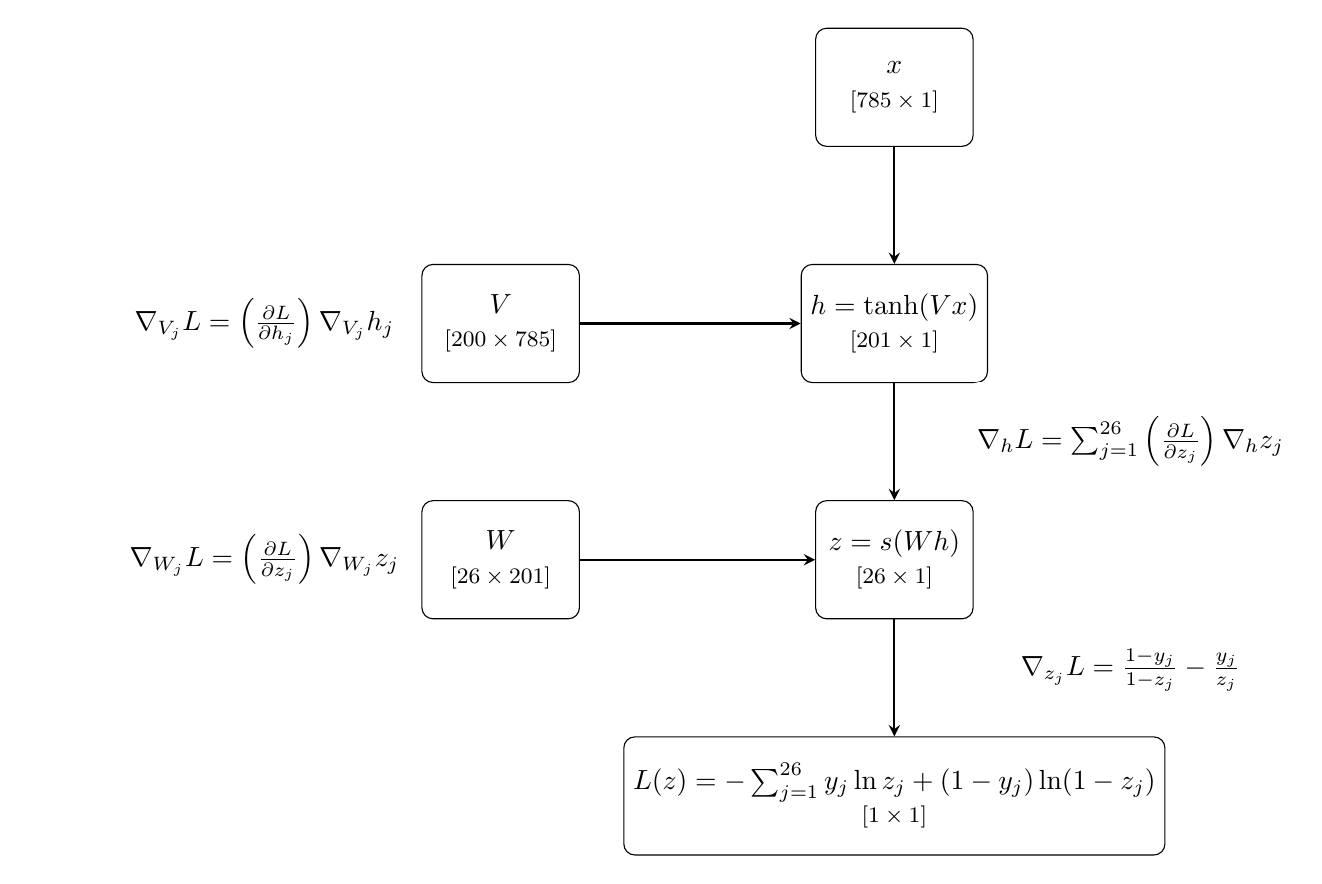
\begin{tikzpicture}[node distance=3cm]

\node (blank) [placeholder] {};
\node (x) [forwardfn, align=center, right of =blank,xshift=7cm] {$x$ \\ \footnotesize$[785\times1]$};
\node (V) [forwardfn, align=center, below of =blank,left of =x,xshift =-2cm] {$V$ \\ \footnotesize$[200\times785]$};
\node (W) [forwardfn, align=center, below of =V] {$W$\\ \footnotesize$[26 \times 201]$};
\node (tanh) [forwardfn, align=center, below of =x] {$h = \tanh(Vx)$ \\ \footnotesize$[201\times1]$};
\node (sigmoid) [forwardfn, align=center, below of=tanh] {$z = s(Wh)$ \\ \footnotesize$[26\times1]$};
\node (loss) [forwardfn, align=center, below of =sigmoid] {$ L(z) = -\sum_{j=1}^{26}{y_j \ln z_j + (1-y_j) \ln(1-z_j)} $\\\footnotesize $[1\times1]$};

\node (gradViL) [backwardfn, left of =V] {$\nabla_{V_j} L =\left(\frac{\partial L}{\partial h_j}\right) \nabla_{V_j} h_j$};
\node (gradWjL) [backwardfn, left of =W] {$\nabla_{W_j} L = \left(\frac{\partial L}{\partial z_j}\right) \nabla_{W_j} z_j $};
\node (gradhL) [backwardfn, right of =tanh, yshift=-1.5cm] {$\nabla_{h} L = \sum_{j=1}^{26}{\left(\frac{\partial L}{\partial z_j}\right) \nabla_{h} z_j }$};
\node (gradzjL) [backwardfn, right of =sigmoid, yshift=-1.4cm] {$\nabla_{z_j} L = \frac{1-y_j}{1-z_j} - \frac{y_j}{z_j} $};

\draw [arrow] (x) -- (tanh);
\draw [arrow] (V) -- (tanh);
\draw [arrow] (tanh) -- (sigmoid);
\draw [arrow] (W) -- (sigmoid);
\draw [arrow] (sigmoid) -- (loss);

\end{tikzpicture}

\-\\
We can substitute the following expressions:\\
\tab$\nabla_{W_j} z_j = z_j(1-z_j)h^T$\tab\footnotesize$[1\times201]$\normalsize\\
\tab$\nabla_{h} z_j = z_j(1-z_j)W_j^T$\tab\footnotesize$[201\times1]$\normalsize\\
\tab$\nabla_{V_j} h_j = \sech^2(V_jx)x^T $\tab\footnotesize$[1\times785]$\normalsize\\

We can also use backpropagation to show:\\
\tab$\nabla_{W_j} L = \left(\frac{1-y_j}{1-z_j} - \frac{y_j}{z_j}\right)\left(z_j(1-z_j) h^T\right)$\tab\footnotesize$[1\times201]$\normalsize\\
\tab$\nabla_{h} L = \sum_{j=1}^{26}{\left(\frac{1-y_j}{1-z_j} - \frac{y_j}{z_j}\right)\left(z_j(1-z_j)W_j^T\right)}$\tab\footnotesize$[201\times1]$\normalsize\\
\tab$\nabla_{V_j} L = \left(\nabla_{h} L\right)_j \sech^2(V_jx)x^T $\tab\footnotesize$[1\times785]$\normalsize\\

To enhance calculation efficiency, we can reduce some of these equations into matrices. First, let $\mathcal{Q}$ be the matrix
$$\mathcal{Q} = \begin{bmatrix}
z_1(1-z_1)\left(\frac{1-y_1}{1-z_1} - \frac{y_1}{z_1}\right)\\
z_2(1-z_2)\left(\frac{1-y_2}{1-z_2} - \frac{y_2}{z_2}\right)\\
\vdots \\
z_{26}(1-z_{26})\left(\frac{1-y_{26}}{1-z_{26}} - \frac{y_{26}}{z_{26}}\right)\\
\end{bmatrix} = \begin{bmatrix}
z_1 - y_1\\
z_2 - y_2 \\
\vdots \\
z_{26} - y_{26} \\
\end{bmatrix}$$

With this, we can reexpress the above equations.\\
(1) \\
\tab$\nabla_{W_j} L = \mathcal{Q}_j h^T $\tab\footnotesize$[1\times201]$\normalsize\\
\tab or
$$ \nabla_{W} L = \begin{bmatrix}
\mathcal{Q}_1 h^T \\
\mathcal{Q}_2 h^T \\
\vdots \\
\mathcal{Q}_{26} h^T \\
\end{bmatrix} = \mathcal{Q}h^T = \mathcal{Q} \otimes h \text{\tab\footnotesize$[26\times201]$\normalsize} $$

(2)\\
\tab$\nabla_{h} L = \sum_{j=1}^{26}{\mathcal{Q}_j W_j^T}$\tab\footnotesize$[201\times1]$\normalsize\\
\tab or
$$ \nabla_{h} L = \begin{bmatrix}
\mathcal{Q}_1 W_1^T + \mathcal{Q}_2 W_2^T + ... + \mathcal{Q}_{26} W_{26}^T\\
\end{bmatrix} $$
$$ \nabla_{h} L = \begin{bmatrix}
W_1^T \mathcal{Q}_1 + W_2^T \mathcal{Q}_2 + ... + W_{26}^T \mathcal{Q}_{26}\\
\end{bmatrix} $$
$$ \nabla_{h} L = \begin{bmatrix}
W_1^T & W_2^T & \hdots & W_{26}^T \\
\end{bmatrix}\begin{bmatrix}
\mathcal{Q}_1 \\
\mathcal{Q}_2 \\
\vdots \\
\mathcal{Q}_{26} \\
\end{bmatrix} = W^T \mathcal{Q} \text{\tab\footnotesize$[201\times1]$\normalsize} $$

(3)\\
Additionally, let
$$ \mathcal{S} = \begin{bmatrix}
\sech^2(V_1 x) \\
\sech^2(V_2 x) \\
\vdots \\
\sech^2(V_{200} x)\\
\end{bmatrix} = \sech^2(Vx) $$
Then, $\nabla_{V_j} L = (W^T \mathcal{Q})_j \sech^2(V_jx)x^T $\tab\footnotesize$[1\times785]$\normalsize\\
\tab or
$$ \nabla_{V} L = \begin{bmatrix}
(W^T \mathcal{Q})_1 \sech^2(V_1 x)x^T \\
(W^T \mathcal{Q})_2 \sech^2(V_2 x)x^T \\
\vdots \\
(W^T \mathcal{Q})_{200} \sech^2(V_{200}x)x^T \\
\end{bmatrix} = \begin{bmatrix}
(W^T \mathcal{Q})_1 \sech^2(V_1 x) \\
(W^T \mathcal{Q})_2 \sech^2(V_2 x) \\
\vdots \\
(W^T \mathcal{Q})_{200} \sech^2(V_{200}x)
\end{bmatrix} x^T $$
$$\nabla_{V} L = \left(\begin{bmatrix}
(W^T \mathcal{Q})_1 \\
(W^T \mathcal{Q})_2 \\
\vdots \\
(W^T \mathcal{Q})_{200} \\
\end{bmatrix} \circ \begin{bmatrix}
\sech^2(V_1 x) \\
\sech^2(V_2 x) \\
\vdots \\
\sech^2(V_{200}x)
\end{bmatrix}\right) x^T = (W^T \mathcal{Q}) \circ \mathcal{S} x^T $$

\newpage
Since we are updating our matrices $V$ and $W$ using stochastic gradient descent, we repeat the following process:

\tab $V,W \leftarrow$ weight matrices initialized randomly from normal distribution with mean $\mu=0$ and $
\sigma^2 = (...)$\\
\tab while (continue = True or $L(z) > 0$) \\
\tab \tab \tab Forward calculation [ $h = \tanh(Vx)$\sep$\rightarrow$\sep$z = s(Wh)$\sep$\rightarrow$\sep$L(z)$ ]\\
\tab \tab \tab Backward calculation to return $\nabla_V L$ and $\nabla_W L$\\
\tab \tab \tab $V \leftarrow V - \epsilon \nabla_V L)$ \\
\tab \tab \tab $W \leftarrow W - \epsilon \nabla_W L$ \\
\tab return $V,W$ \\

where, using our derived equations from above, the update rules are more specifically\\
\tab \tab \tab \tab $V \leftarrow V - \epsilon(W^T \mathcal{Q}) \circ \mathcal{S} x^T $\\
\tab \tab \tab \tab $ W \leftarrow W - \epsilon(\mathcal{Q} \otimes h). $



\newpage
%%%%%%%%%%%%%%%%%%%%%%%%%%%%%%%%%% PROBLEM 2 %%%%%%%%%%%%%%%%%%%%%%%%%%%%%%%%%%
\section*{Problem 2}

\subsection*{Implemenation \& Results:}
1) \textbf{Hyperparameters}\\
\tab \tab Manually tested values of learning rate $\epsilon$ between 1 and and $1\times10^{-5}$. Settled on 0.1 as an optimal value.

2) \textbf{Training Accuracy}\\
\tab \tab 88.94\% training accuracy was achieved after 20 epochs of stochastic gradient descent training.

3) \textbf{Validation Accuracy}\\
\tab \tab 86.63\% validation accuracy was achieved on the 20\% of data that was initially withheld.

4) \textbf{Loss vs. Iterations}\\
\tab \tab (...)

5) \textbf{Kaggle}\\
\tab \tab Display Name: mitch
\tab \tab Score: 0.87106

6) \textbf{Code}\\
\tab \tab See appendix for full implementation in NeuralNet class



\newpage
%%%%%%%%%%%%%%%%%%%%%%%%%%%%%%%%%% PROBLEM 3 %%%%%%%%%%%%%%%%%%%%%%%%%%%%%%%%%%
\section*{Problem 3}

\subsection*{Visualization}

Correctly classified images:\\
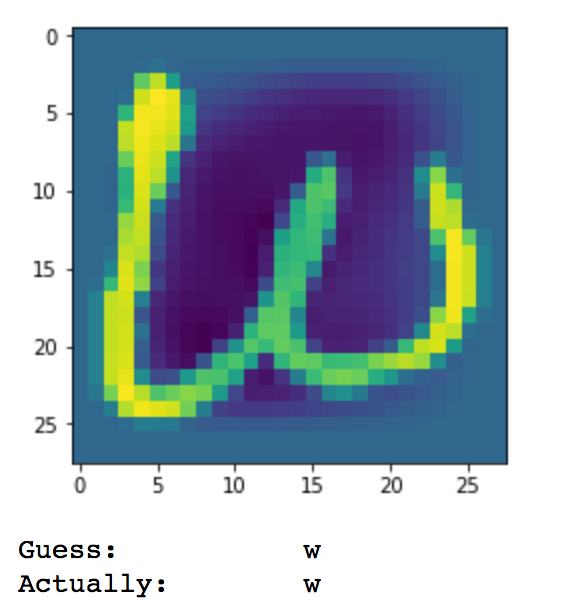
\includegraphics[width=3cm]{correctclass01.png}
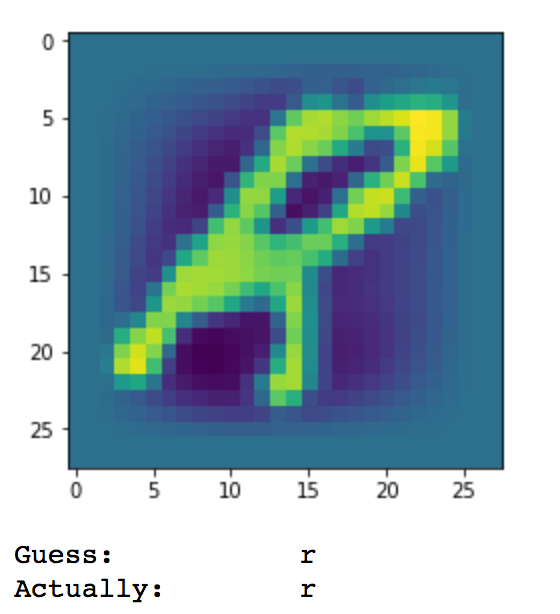
\includegraphics[width=3cm]{correctclass02.png}
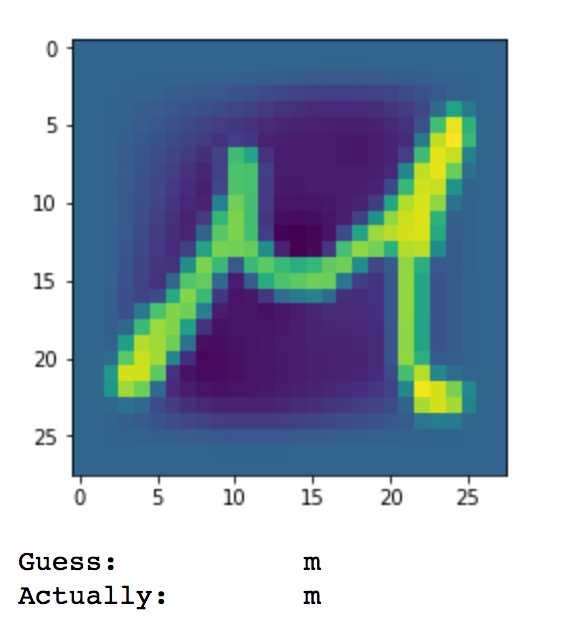
\includegraphics[width=3cm]{correctclass03.png}
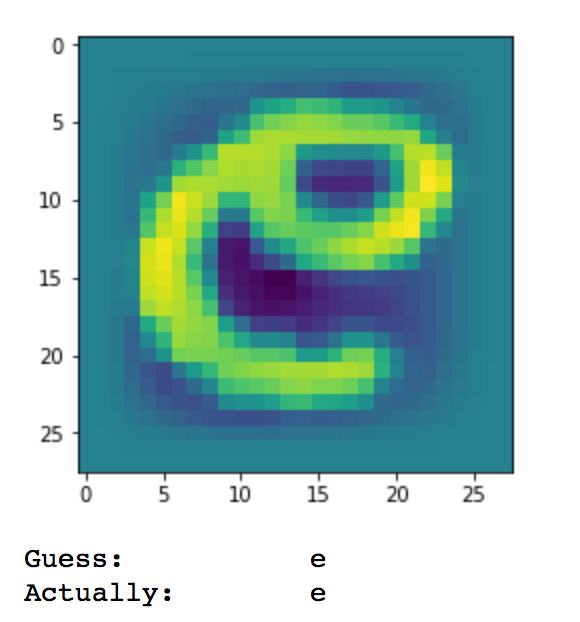
\includegraphics[width=3cm]{correctclass04.png}
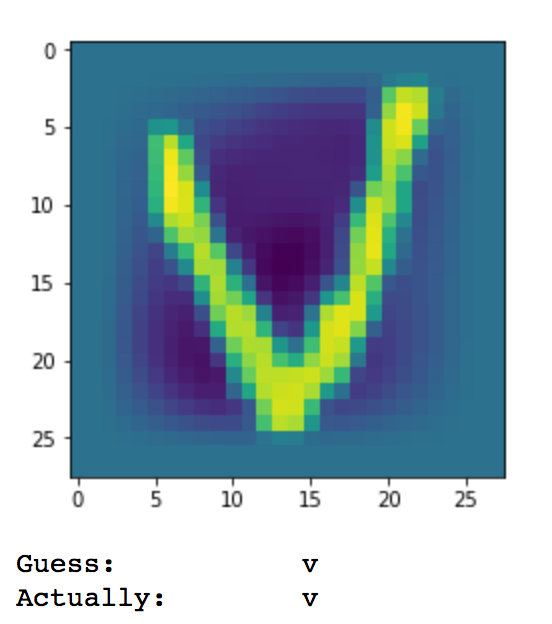
\includegraphics[width=3cm]{correctclass05.png}

Incorrectly classified images:\\
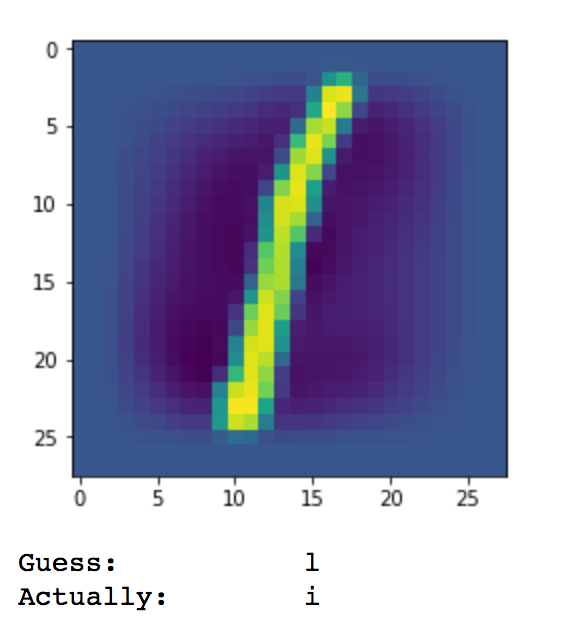
\includegraphics[width=3cm]{incorrectclass01.png}
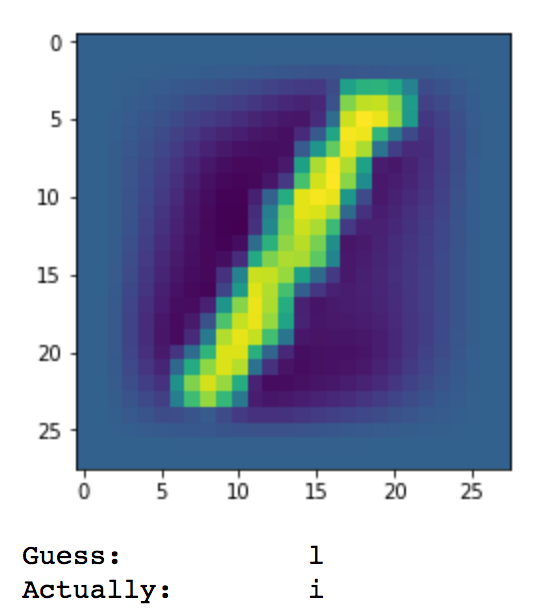
\includegraphics[width=3cm]{incorrectclass02.png}
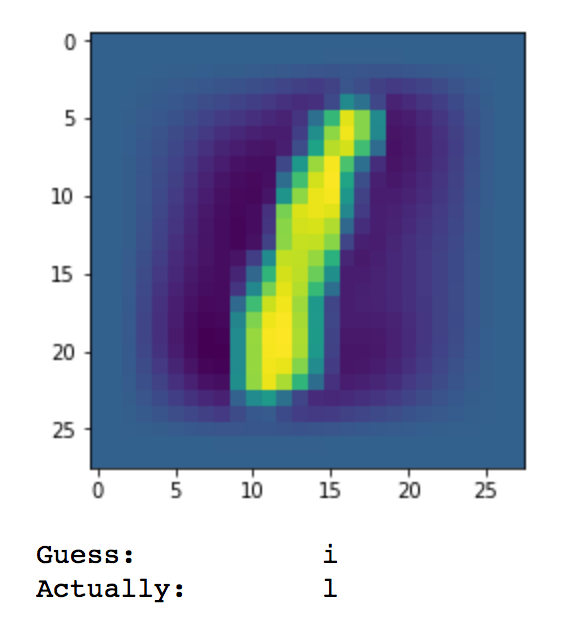
\includegraphics[width=3cm]{incorrectclass03.png}
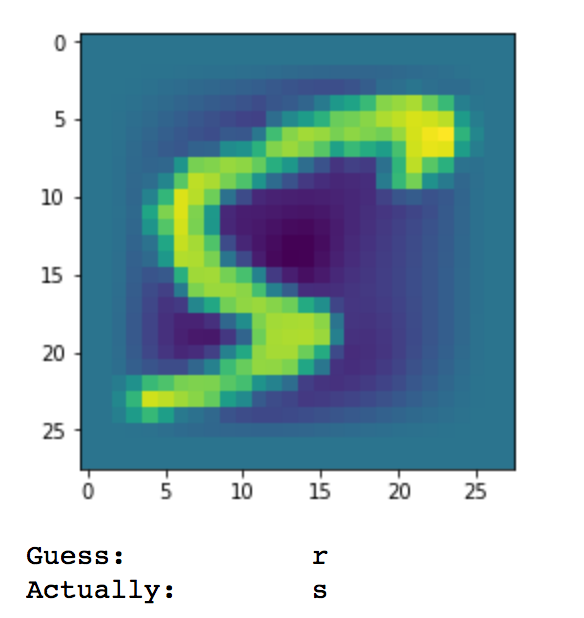
\includegraphics[width=3cm]{incorrectclass04.png}
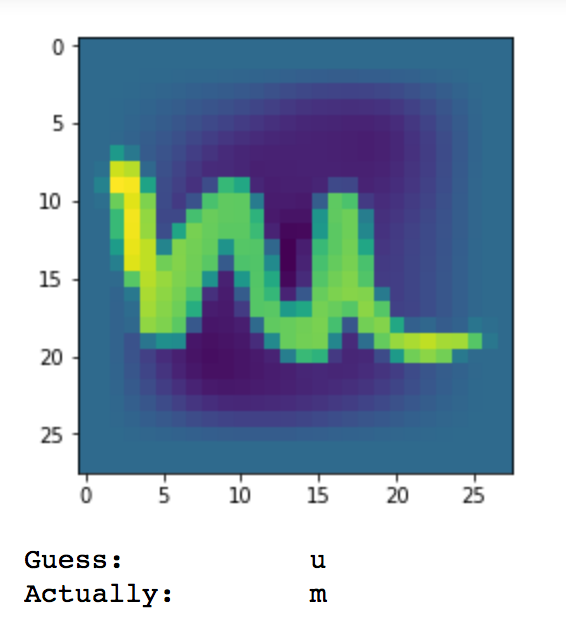
\includegraphics[width=3cm]{incorrectclass05.png}



\newpage
%%%%%%%%%%%%%%%%%%%%%%%%%%%%%%%%%% PROBLEM 4 %%%%%%%%%%%%%%%%%%%%%%%%%%%%%%%%%%
\section*{Problem 4}

No extra bells and whistles were tested, though the neural network was designed to be flexible.
The code currently operates using stochastic gradient descent, though it is designed to be able to take in multiple points (or the complete dataset) for easy conversion to batch/mini-batch gradient descent.

Furthermore, the modular structure allows the neural network to be adapted for any number of layers and any number of hidden units per layer. 
To do this, the code takes in the following sequences as arguments: layers, number of hidden units per layer, and activation functions per layer. 
Two modules are necessary to run this code, one containing activation functions to be included in the input sequence, and one containing a "gradient calculator" class which computes appropriate gradients for the desired neural network configuration.



\newpage
%%%%%%%%%%%%%%%%%%%%%%%%%%%%%%%%%% APPENDIX %%%%%%%%%%%%%%%%%%%%%%%%%%%%%%%%%%
\section*{Appendix}

\lstinputlisting[language=Python,basicstyle=\ttfamily\scriptsize]{"/Users/mitch/Documents/Cal/2_2017_Spring/COMPSCI 289A - Intro to Machine Learning/HW06/Code/neuralnet.py"}

\newpage
\lstinputlisting[language=Python,basicstyle=\ttfamily\scriptsize]{"/Users/mitch/Documents/Cal/2_2017_Spring/COMPSCI 289A - Intro to Machine Learning/HW06/Code/gradients.py"}

\-\\
\-\\
\-\\
\-\\
\lstinputlisting[language=Python,basicstyle=\ttfamily\scriptsize]{"/Users/mitch/Documents/Cal/2_2017_Spring/COMPSCI 289A - Intro to Machine Learning/HW06/Code/activationfns.py"}




\end{document}




